\noindent  Es una representaci\'on pict\'orica de conjuntos donde los conjuntos est\'an representados por \'areas cerradas en el plano.
    \begin{center}
        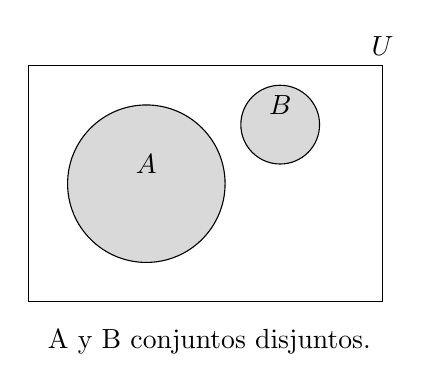
\begin{tikzpicture}
                % Conjunto universal
                \draw[fill=white!20] (-1.5,-1.5) rectangle (3,1.5) node[above] {$U$};
                                     
                % Conjunto B
                \draw[fill=gray!30] (1.7,0.75) circle (0.5cm) node[above] {$B$};
                % Conjunto A
                \draw[fill=gray!30] (0,0) circle (1cm) node[above] {$A$};
                % Título
                \node at (0.8,-2) {A y B conjuntos disjuntos.};
            \end{tikzpicture}
    \end{center}